\documentclass{standalone}
\usepackage{tikz}
\usetikzlibrary{arrows,shapes,chains,matrix,positioning,scopes,patterns,calc}
\usepackage{color}

\begin{document}

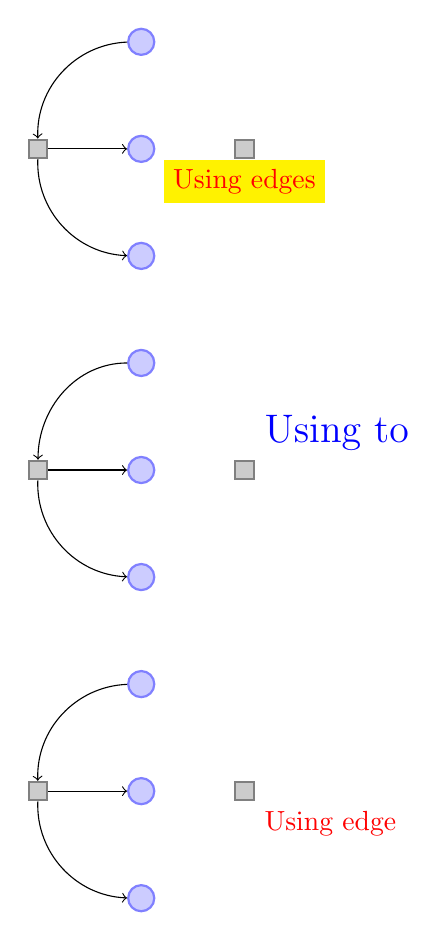
\begin{tikzpicture}
 [place/.style={circle,draw=blue!50,fill=blue!20,thick},
   transition/.style={rectangle,draw=black!50,fill=black!20,thick}]
   
  \node[place] (waiting){};
  \node[place] (critical) [below=of waiting] {};
  \node[place] (semaphore) [below=of critical]{};
  
 
  \node[transition] (leave critical) [right=of critical,label={[red,fill=yellow]below: Using edges}] {};
%  For label in red: First, he can redefine the every label style. Second, he can add options to the label’s node. These options are given following the label=, so he would write label=[red]above:$s\le3$. However, this does not quite work since TEX thinks that the ] closes the whole option list of the semaphore node. So, Hagen has to add braces and writes label={[red]above:$s\le3$}. Since this looks a bit ugly, Hagen decides to redefine the every label style: \begin{tikzpicture}[every label/.style={red}].
  \node[transition] (enter critical) [left=of critical]  {}
    edge [->]               (critical)
    edge [<-,bend left=45]  (waiting)
    edge [->,bend right=45] (semaphore);
    
    
    
 \node[place] (waiting1)[below =of semaphore]{};
  \node[place] (critical1) [below=of waiting1] {};
  \node[place] (semaphore1) [below=of critical1]{};
  
  \node[transition] (leave critical1) [right=of critical1,label={[blue,font=\Large]north east: Using to}] {};
  \node[transition] (enter critical1) [left=of critical1]  {};
  \draw [->] (enter critical1) to                 (critical1);
  \draw [->] (waiting1)        to [out=180,in=90] (enter critical1);    
  \draw [->] (enter critical1) to [bend right=45] (semaphore1);


 \node[place] (waiting2)[below =of semaphore1]{};
  \node[place] (critical2) [below=of waiting2] {};
  \node[place] (semaphore2) [below=of critical2]{};
  
  \node[transition] (leave critical2) [right=of critical2,label={[red]south east: Using edge}] {};
 \node[transition] (enter critical2) [left=of critical2]  {}
    edge [->]               (critical2)
    edge [<-,bend left=45]  (waiting2)
    edge [->,bend right=45] (semaphore2);

\end{tikzpicture}
\end{document}